\section{Git болон GitHub}
Git бол өнөө үеийн хөгжүүлэгчдийн ямар нэгэн байдлаар заавал хэрэглэдэг Version Control System (VCS) технологийн нэг билээ. Ажилд орох, багаар хөгжүүлэлт хийх, зайнаас ажиллах, хөгжүүлэлтийн түүхээ хадгалах, удирдах гэх мэт олон шалтгааны улмаас хөгжүүлэгчид ашигладаг. 2005 онд Linus Torvalds (linux-ийн зохион бүтээгч гэдгээрээ алдартай) болон Junio C Hamano нар анх Git технологийг өөрсдийн linux kernel-ийн хөгжүүлэлтийн явцдаа зохион бүтээжээ. Ул шалтгаан нь тэдэнд open-source VCS-ийн хэрэгцээ гарснаас улбаатай гэж тэмдэглэсэн байдаг.
Git-д дараах чухал ойлголтууд байдаг. Үүнд,
\begin{itemize}
    \item Branching (Салбарлах)
    \item Merging (Нэгтгэх)
    \item Commits
    \item Staging Area
\end{itemize}
\par
Branching бол хөгжүүлэгчдийг тухайн төслийн олон хувилбарыг \emph{салбарлуулж} параллель байдлаар ажиллах боломжийг олгодог. Үүний тусламжтайгаар хөгжүүлэгчид гол кодоо өөрчилж алдаа гаргахгуйн тулд салбарлалтын аргыг ашиглаж бусад хувилбар кодуудаа туршиж үздэг. Жишээ нь, "Khuur"-ийн нэмэлт нэвтрэх болон бүргүүлэх хэсгийн кодыг хөгжүүлэхдээ гол ажилж буй \emph{Branch} (мөчир) дээрх кодыг өөрчлөхийн оронд тусдаа салбар мөчир үүсгэж түүн дээрээ хөгжүүлэлтээ хийнэ гэсэн үг юм. Нэг ёсондоо, гол кодын хэрэгжүүлэлтэд алдаа гарна гэж санаа зовох шаардлагагүй болно. \par
Merging буюу нэгтгэх ойлголт нь дээрх салбарласан мөчрүүдийг хооронд нь нийлүүлэх тохиолдолд хэрэглэдэг арга. Тэгэхээр салбарлах ойлголттой нягт холбоотой юм. Өмнөх жишээн дээр дурдсан "Khuur"-ийн хувьд нэвтрэх хэсгийн хөгжүүлэлт дуусаж хангалттай чанартай болсон гэж үзвэл гол мөчир кодтойгоо шууд нэгтгэж нэвтрэх хэсэг гол кодтой нэгдэнэ.\par
Төслийн хөгжүүлэлтийн явцад хөгжүүлэгчид одоогийн бичсэн кодоо дараа нь харах \\ боломжтой түүх байдлаар хадгалах хэрэгцээ үүсдэг. Үүнийг Git \emph{commit}-ийн тусламжтайгаар шийддэг. Түүх болгон хадгалахыг хүссэн үедээ уг төслийг \empth{commit} хийснээр төслийн фолдерийн байдлыг тэр чигээр нь зураг авч байгаатай адил хадгалдаг. Ингэснээр ирээдүйд уг код дээр эргэж ирэх шаардлага гарвал \emph{commit} түүхээ харахад л хангалттай. \par
Харин Staging Area нь commit хийхээс өмнөх хадгалахыг хүссэн файл болон фолдеруудын жагсаалт юм. Өөрөөр хэлбэл, төслийн аль файлуудыг түүх болгон үлдээхийг хэрэглэгч өөрөө тодорхойлох боломжтой болж байгаа юм. \par


GitHub бол Git-г ашигладаг веб платформ юм. Бусадтай хамтарч ажиллах, төслөө хадгалах, прожект менежмент, continuous integration, болоод бусдын төслийг харах, судлах, хуулбарлах гэх мэт маш олон үйлчилгээг үзүүлдэг. Ихэнхдээ багаар ажиллах, код хадгалахад хөгжүүлэгчид ихэвчлэн хэрэглэдэг. Гол онцлогуудаас дурдвал,
\begin{itemize}
    \item Repository: Гит репозиторуудыг хадгалж, тэдгээртэй харьцахад хялбар UI
    \item Pull request: Багаар ажиллаж байхдаа нэг нэгнийхээ кодыг хянах байдлаар хийсэн өөрчөлтүүдийг бусад гишүүдээр эсвэл хариуцсан мэргэжилтнээр нь хянуулж бусад мөчиртэй нэгтгэх хүсэлт илгээж болдог.
    \item Forks: Төсөлд ямар ч нөлөө үзүүлэхгүйгээр хуулбарлаж хөгжүүлэлт хийх боломж.
    \item Issues: Алдаа, bug болон сайжруулалтыг хянах нэг арга.
    \item Actions: Хөгжүүлэх, тестлэх, байршуулах ажлын урсгалыг автоматжуулдаг.
\end{itemize}
\section{Dart}
Dart\footnote{Dart албан ёсны вэбсайт \url{https://dart.dev/}} программчлалын хэл нь Javascript-ийг орлуулах зорилготой Google компанийн хөгжүүлсэн хэл билээ. Анх 2011 оны 10 сард олон нийтэд зарлагдаж байсан энэхүү хэл нь өнөөдөр cross-platform буюу нэг кодоор бүх платформ дээр ажилдаг бүтээгдэхүүн хөгжүүлэхэд өргөн хэрэглэгддэг. Өөрөөр хэлбэл, дарт код болон Flutter-ийн тусламжтайгаар windows, linux, macos, android, ios зэрэг платформууд дээр шууд ажиллах боломжийг нээж өгсөн юм. Хэдий анх Javascript хэлийг орлох зорилгоор хараахан амжилт олж чадаагүй ч ялангуяа мобайл хөгжүүлэлтэд хөгжүүлэгчид өргөн хэрэглэж байна.

Dart-ийн давуу тал нь хөгжүүлэлтийн явцад алдаагаа олж мэдээлэлдэг. Энэ нь хамгийн түгээмэл хэрэглэдэг Javascript хэлэнд байдаггүй сул талыг нөхсөн том онцлог. Мөн Dart эх код руу Ahead-Of-Time (AOT) хөрвүүлэлтийг дэмждэг нь гар утасны программуудад чухал ач холбогдолтой өндөр гүйцэтгэлийг баталгаажуулж, Just-In-Time (JIT) эмхэтгэлийн тусламжтайгаар "hot reload" боломжийг олгодог бөгөөд энэ нь ялангуяа Flutter ашиглах үед программуудыг хурдан хөгжүүлэх боломжийг олгодог. Үүнээс гадна уг хэлний синтакс нь орчин үеийн хэлнүүдийн адил сурч ойлгоход маш хялбар байдаг.
Dart хэл дээр дараах байдлаар "Hello, world!" программыг бичдэг.
\begin{lstlisting}[language=Dart, caption=Dart хэл дээрх анхны программ бичилтийн синтакс, frame=single]
void main() {
  print('Hello, World!');
}
\end{lstlisting}

\section{Flutter}
Dart хэлийг Flutter\footnote{Flutter албан ёсны вэбсайт \url{https://flutter.dev/}} фреймворкгүйгээр төсөөлөхөд бэрх. 2015 онд анх Google компаниас open-source байдлаар гаргасан фреймворк нь нэг баазаас window, macos, linux, web, android, ios платформуудад зориулсан программ хөгжүүлэхэд хэрэглэгддэг. Ялангуяа гар утасны программ хөгжүүлэлтэд нэлээн нэр хүндтэй юм. Түүний гол онцлогуудаас дурдвал,
\begin{itemize}
    \item Flutter-ийн хамгийн анхаарал татахуйц шинж чанаруудын нэг нь кодыг нэг удаа бичиж, олон платформ дээр ажиллуулж, цаг хугацаа, хүч хэмнэдэг чадвар юм.
    \item Flutter программууд нь эх кодруу хөрвүүлэлт хийдэг бөгөөд энэ нь өндөр гүйцэтгэл, ойр мэдрэмжийг өгдөг.
    \item Flutter нь Material Design болон Cupertino-ийн зааврйг дагаж мөрддөг, урьдчилан боловсруулсан олон төрлийн виджетүүдийг санал болгодог бөгөөд хөгжүүлэгчдэд төвөгтэй UI-г хялбархан үүсгэх боломжийг олгодог.
\end{itemize}
Анхлан суралцагчдад Flutter их ойлгомжгүй санагдаж цаг хугацаа авах нь элбэг тохиолддог ч нэг учрыг нь олчихвол миний хувьд их ойлгомжтой амархан санагддаг. Дараах код нь Flutter-ийг ашиглан товч дээр товшин тоо нэмдэг энгийн программыг хэрхэн программчилдгыг харууллаа.
\begin{lstlisting}[language=Dart, caption=Flutter "Counter" жишээ код, frame=single]
import 'package:flutter/material.dart';

void main() {
  runApp(MyApp());
}

class MyApp extends StatelessWidget {
  @override
  Widget build(BuildContext context) {
    return MaterialApp(
      home: Scaffold(
        appBar: AppBar(title: Text('Flutter Example')),
        body: MyHomePage(),
      ),
    );
  }
}

class MyHomePage extends StatefulWidget {
  @override
  _MyHomePageState createState() => _MyHomePageState();
}

class _MyHomePageState extends State<MyHomePage> {
  int _counter = 0;

  void _incrementCounter() {
    setState(() {
      _counter++;
    });
  }

  @override
  Widget build(BuildContext context) {
    return Center(
      child: Column(
        mainAxisAlignment: MainAxisAlignment.center,
        children: <Widget>[
          Text('You have pushed the button this many times:'),
          Text('$_counter', style: TextStyle(fontSize: 24)),
          ElevatedButton(
            onPressed: _incrementCounter,
            child: Text('Increment'),
          ),
        ],
      ),
    );
  }
}
\end{lstlisting}
Үр дүн:
\clearpage
\begin{figure}[h]
	\centering
	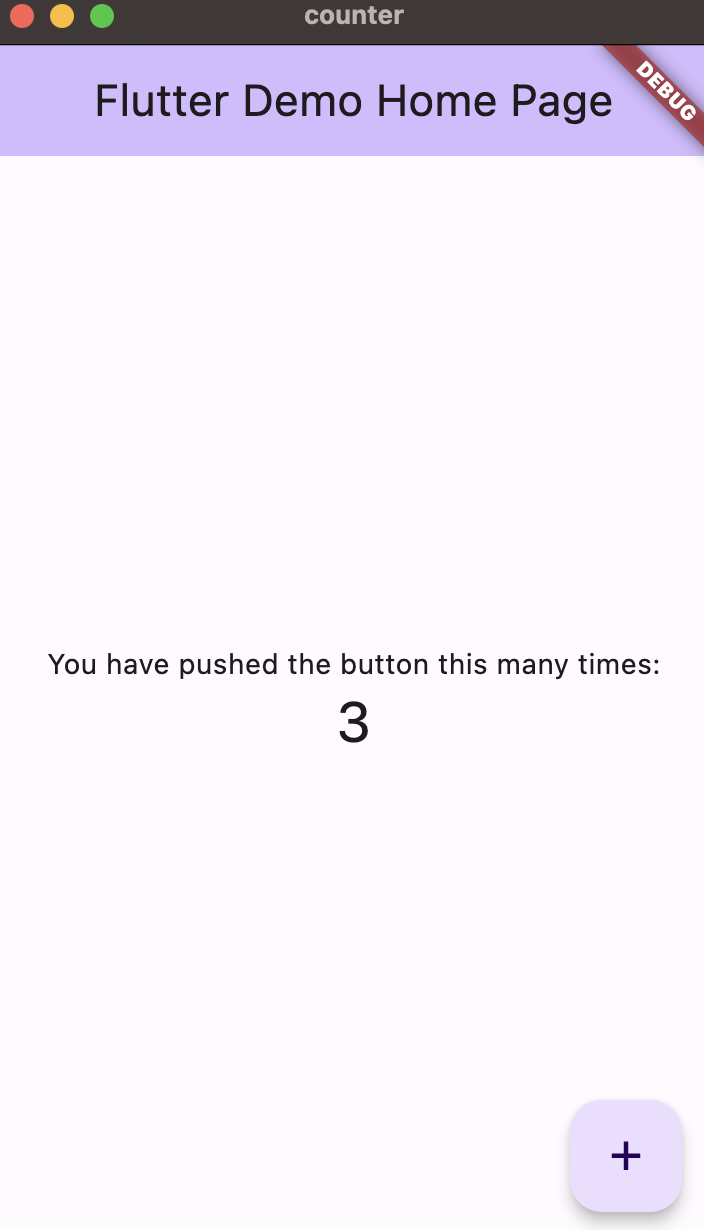
\includegraphics{images/counter.png}
	\caption{Counter жишээ код}
	\label{fig:modalform}
\end{figure}
\clearpage
Дээрх кодны жишээ виджетүүдийг маш олон газар ашигласан байна. Жишээ нь,
\begin{lstlisting}
  Widget build(BuildContext context) {
    return MaterialApp(
      home: Scaffold(
        appBar: AppBar(title: Text('Flutter Example')),
        body: MyHomePage(),
      ),
    );
  }
\end{lstlisting}
энэ методын хувьд \emph{MaterialApp(), Scaffold(), AppBar(), MyHomePage()} зэрэг нь бүгд виджетийн нэг жишээ юм.

\section{AWS}
Amazon Web Services\footnote{AWS албан ёсны вэбсайт \url{https://aws.amazon.com/}} (AWS) нь Амазон компаниас хангадаг үүлэн тооцооллын платформ бөгөөд бизнес болон хувиараа хөгжүүлэгчдэд үүлэн дээр программ ажиллуулах боломжийг олгодог өргөн хүрээний нөөц, үйлчилгээг санал болгодог. 2006 онд үүссэн AWS нь үүлэн тооцооллын салбарт топ 1-т жагсаж, өргөтгөх боломжтой, найдвартай, хэмнэлттэй тооцооллын шийдлүүдээр хангасаар ирсэн. Өдгөө AWS-ын 200 гаруй үйлчилгээг дараах ангилалд хувааж болно. Үүнд:
\begin{itemize}
    \item Тооцоолох: Хэрэглэгчдэд виртуал сервер түрээслэх, тооцооллын ажил удирдах боломжийг олгодог үйлчилгээ байдаг. Жишээ нь, EC2 (Elastic Compute Cloud).

    \item Хадгалах: Өргөтгөх боломжтой объект хадгалахад зориулсан S3 (Simple Storage Service), блок хадгалахад зориулсан EBS (Elastic Block Storage) зэрэг функцууд.

    \item Өгөгдлийн сан: SQL мэдээллийн санд зориулсан RDS (Relational Database Service), NoSQL шийдэлд зориулсан DynamoDB санал болгодог.

    \item Контентийн хүргэлт ба CDN: Amazon CloudFront нь контентыг дэлхий даяар түгээх Content Delivery Network-ийн үүрэг гүйцэтгэдэг.

    \item Сүлжээ: VPC (Virtual Private Cloud) нь хэрэглэгчдэд AWS экосистем дотор тусгаарлагдсан сүлжээ үүсгэх боломжийг олгодог.

    \item Машин сургалт ба хиймэл оюун ухаан: Машин сургалтын загварт зориулсан SageMaker, байгалийн хэлээр боловсруулахад зориулсан Comprehend зэрэг үйлчилгээ багтана.

    \item Хөгжүүлэгчийн хэрэгслүүд: CI/CD дамжуулах pipeline болон Cloud9-д зориулсан CodeBuild болон CodeDeploy-ийг онлайн IDE болгон хангадаг.

    \item IoT: AWS IoT Core нь эд зүйлсийн интернет төхөөрөмжүүдийг нэгтгэх боломжийг олгодог.

    \item Аюулгүй байдал ба тодорхойлолт: IAM (Identity and Access Management) нь хандалтын хяналтыг зохицуулдаг.

    \item Аналитик: Том өгөгдлийн шинжилгээнд зориулсан EMR, бодит цагийн өгөгдөл дамжуулах Kinesis, бизнесийн аналитикт зориулсан Quicksight зэргийг багтаасан.
\end{itemize}

Уг технологи нь өргөтгөх боломжтой, өртөг хэмнэлттэй, өргөн хүрээний үйлчилгээ, найдвартай байдал, найдвартай хамгаалалтын функцүүдийн давуу талыг санал болгодог бөгөөд энэ нь янз бүрийн тооцооллын хэрэгцээнд цогц шийдэл болж чаддаг. Гэсэн хэдий ч энэ нь гэнэтийн зардалд хүргэж болзошгүй төлбөр, олон тооны үйлчилгээг сурах хугацаа, гадагшаа өгөгдөл дамжуулахад гарах зардал зэрэг сул талуудтай. Мэргэжилтэн эсвэл хяналт байхгүй бол маш олон төлбөрийн болоод хангамжийн эрсдэлүүдтэй тулгарах өндөр эрсдэлтэй юм.